%++++++++++++++++++++++++++++++++++++++++
% Don't modify this section unless you know what you're doing!
\documentclass[a4paper,12pt]{report}
\usepackage[tocflat]{tocstyle}
\usepackage[toc,page]{appendix}
\usepackage{appendix}
\usetocstyle{standard}
\usepackage{titlesec}
\usepackage{lipsum}
\renewcommand{\abstractname}{\large{\uppercase{Abstract}}}
\renewcommand\contentsname{\uppercase{Table of contents}}
\renewcommand{\listtablename}{\uppercase{List of Tables}}
\renewcommand{\listfigurename}{\uppercase{List of Figures}}
\renewcommand{\bibname}{REFERENCES}
\titleformat{\chapter}
{\normalfont\large\bfseries\centering\uppercase}
    {}{0.5em} {}
\usepackage{tabularx} % extra features for tabular environment
\titleformat{\section}{\normalsize\bfseries\uppercase}{\thesection}{0.5em}{}
\titleformat*{\subsection}{\normalsize\bfseries}
\titlespacing*{\chapter}{0.00in}{-0.5in}{5mm}
\usepackage{amsmath}
\usepackage{mathptmx}
\usepackage{float}% improve math presentation
\usepackage{graphicx} % takes care of graphic including machinery
\usepackage{chemformula}
\usepackage[lmargin=1.5in, rmargin= 1in, bmargin=1in, tmargin=1in, a4paper]{geometry} % decreases margins
\usepackage{cite} % takes care of citations
\usepackage{gensymb}
\usepackage[final]{hyperref} % adds hyper links inside the generated pdf file
\hypersetup{
	colorlinks=true,       % false: boxed links; true: colored links
	linkcolor=blue,        % color of internal links
	citecolor=blue,        % color of links to bibliography
	filecolor=magenta,     % color of file links
	urlcolor=blue         
}

%++++++++++++++++++++++++++++++++++++++++

\linespread{1.4}
\newcommand{\mychapter}[2]{
    \setcounter{chapter}{#1}
    \setcounter{section}{0}
    \setcounter{table}{0}
    \setcounter{figure}{0}
    \chapter*{#2}
    \addcontentsline{toc}{chapter}{#2}
}
\begin{document}
\title{CSE-344 SYSTEM PROGRAMMING\newline FINAL PROJECT}
\author{GÖKHAN HAS - 161044067}
\date{June 28, 2020}
\maketitle
\pagenumbering{roman}

\newpage


\mychapter{1}{CSE-344 SYSTEM PROGRAMMING FINAL PROJECT}
\pagenumbering{arabic}
\paragraph{1. INTRODUCTION\newline} 
The final project was a mixture of topics we learned throughout the semester. I also reinforced what I learned using everything I learned throughout the period. I solved the processes using daemon, using TCP sockets, making thread pool, transferring data between threads using pipe, and synchronization using mutexes and condition variables. 

\paragraph{2. SERVER\newline}
The server part is located in "161044067\_final.c" file. As is known, it is the main part of the assignment. There are struct definitions for the thread pool at the beginning. Then, global variables used in the code are defined. The functions used are described here. The purpose of the functions is written in the code as a comment line. The purpose of the functions will be explained in the "used functions" section on the following pages.

\paragraph{}
When the program runs, argument control is done at first. For the server part, the arguments -i, -p, -o, -s, -x and -r are checked. If the user enters wrong arguments, the program prints a sample with correct usage and prints out what the arguments will be used for. It is also important that some arguments are numbers, such as portnumber (-p). It is checked whether these consist of numbers. If the user does not enter numbers in these arguments, the program warns that it needs to enter numbers.

\begin{figure}[h!]
\centering
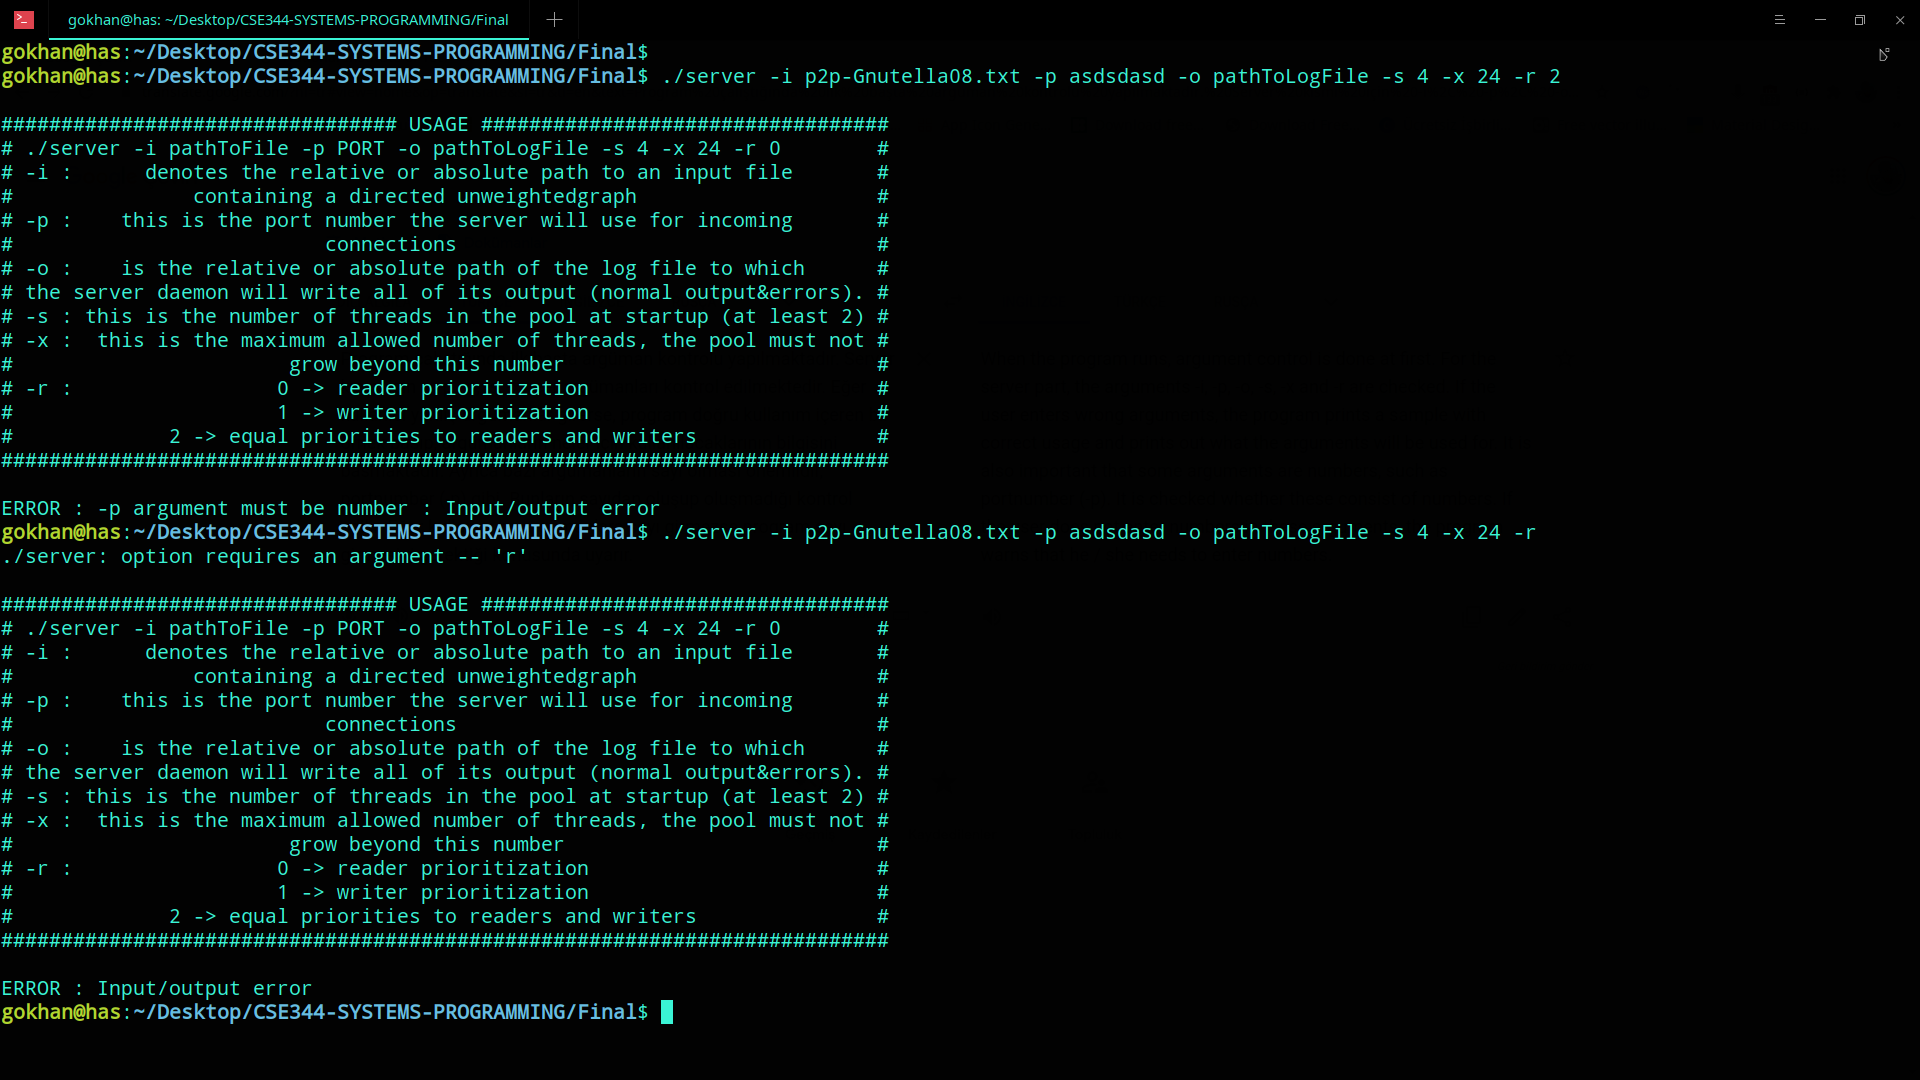
\includegraphics[scale=0.25]{1_wrongınput.png}
\caption{Wrong Input Test}
\label{fig:compile}
\end{figure}

\newpage
\paragraph{}
In the final project, SIGINT, ie CTRL C signal is requested to be catched. That's why I defined it at the beginning of the main using the sigaction structure and making the necessary assignments. It was necessary to define this structure. If it were done using the normal signal function, there would be a problem with the socket. The program would not close. So this structure was used and a signal\_handler function was written. This function assigns 1 to the variable SIGINT\_FLAG. The rest of the server has controls based on this flag.

\paragraph{}
After the argument checks are done, the deamon process is created. After that, the log file opens, if no log file is available. If a file with the same name is found before, it is added to the end. Because it is tried to open in "a +" mode.

\paragraph{}
After the above processes are completed, the graph is initialized. How many nodes are there, one-dimensional array with so many elements is created. Thus, it is possible to access that node in O (1) time. When adding an edge, the next nodes of the nodes in that index are used. Structure is defined in "graph.h" file. Below is a shaped explanation of the graph structure I have set up. It usually takes a short time to read the input file and load the graph. Sometimes it takes a long time when working with Valgrind.

\begin{figure}[h!]
\centering
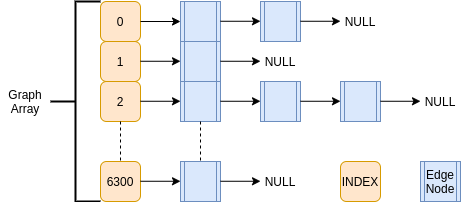
\includegraphics[scale=0.75]{2_graph.png}
\caption{Graph Structure}
\label{fig:compile}
\end{figure}

\paragraph{}
Thread pool is created according to the min or maximum values entered by the user. A "Threadpool\_t" structure contains first and last thread structures that point you to maxCapacity, ids array, conditionArr, mutexes, as well as two "OneThread" structures. The purpose is to make the add part in O (1) time in the function that performs the resize operation. This process is possible and effective since the last thread is held with "last". The "OneThread" structure contains the thread of id, isWorking, socket\_fd, source, destination, pipe, pthread\_t and nextThread, which also holds the address of the next thread, "OneThread *".

\begin{figure}[h!]
\centering
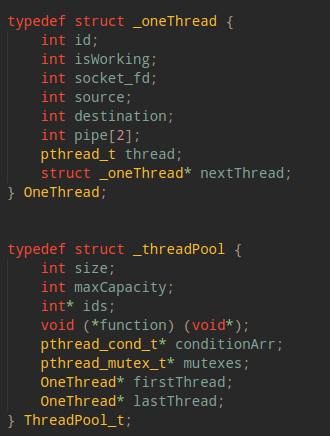
\includegraphics[scale=0.75]{3_threadpool.png}
\caption{ThreadPool\_t Structure}
\label{fig:compile}
\end{figure}

\paragraph{}
At first the thread is created as many as the number -s argument. It is then done in a separate thread using the reinitializeThreadPool function. If Main says that new threads need to be loaded, this function works. Communication of these two functions was done using pipes. The function does not work until data is written to pipe. Since the last thread is kept in the thread pool, adding in O (1) time is done in this function (reinitializeThreadPool). Main continues to work.

\paragraph{}
Cache structure should have been very efficient. So I implemented it graph structure. I have a CacheEntry array. This actually holds the CacheEntry structure as much as the number of nodes. This includes structures of the cacheSize, first and CacheBlock * data types. For example, the user wants to find the path from 1200 to 6200. First, by making cache [1200], I can reach which node from 1200 in O (1) time. Then, by doing cache [1200] .nextBlock-last, I check if the value of 6200 is equal to this value. If it is equal, I return it by taking the int array in the CacheBlock structure. Thus, searching in cache is very fast. In the beginning, I assign values to -1. For example, you want to search from 1500 to 8000. But cache has not gone 1500 vertex anywhere. Since the value is -1, it is checked once.

\newpage
\begin{figure}[h!]
\centering
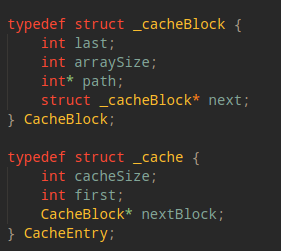
\includegraphics[scale=1.0]{4_cache1.png}
\caption{Cache Structure}
\label{fig:compile}
\end{figure}

\paragraph{2.1. Used Function In Server Side\newline}
\begin{itemize}
    \item void errorExit(char* error) : Print error message and exit gracefully.
    \item void printUsage() : Print program usage if the user entered wrong input.
    \item int controlIfArgumentDigit(char* argumentValue) : Same arguments must be digit, fx portnumber, control these arguments.
    \item int controlDuplicateServer() : The server should not run twice at the same time.
    \item size\_t getMaksimumNodeNumber(char* fileName, int* edgeNumber) : Returns the maximum number of nodes in the graph.
    \item int readFileAndInitializeGraph(char *fileName, Graph* graph, int nodeNumber, int edgeNumber) : The graph is initialized by reading the file line by line.
    \item void printStartMessageToLogFile(char* iVal, char* oVal) : When the server runs for the first time in the log file, the messages are printed. Only timestamp is placed in the last of these messages.
    \item int BFSalgorithm(Graph* graph, int source, int destination, int* visitedArr, int* path, int* pathIndex, int* count, int maxEdge) : It is the function that calculates the classical BFS algorithm. With the help of the queue, bfs is calculated. At the level level, it is not always possible to go to the next level before the upper level ends. If there is an edge between nodes, the shortest is always found.
    \item void getPath(Queue * queue, int* path, int destination, int maxNode, int kIndex, int count) : According to the BFS algorithm, the path between the nodes must be found and saved in the cache or sent to the clients.
    \item void* reinitializeThreadPool(void* argument) : It is the thread function that changes the reputation of the thread pool. Adding to threadpool is done in this function.
    \item void* response\_threads(void* argument) : It is the main function where threads will work. Incoming requests are calculated here, if any, search or add operation in cache.
    \item void initializeThreadPool() : This is the function that initializes threadpool initially.
    \item void freeThreadPool() :  Resources used for threadpool are free.
    \item OneThread* returnEmptyThread() : Returns the thread structure not working.
    \item int getRunningThreadCount() : Returns the number of threads running.
    \item void initializeBFSarrays(int* path, int* visitedArr) : Prepares the variables required for BFS.
    \item void printPathFromDataBase(CacheBlock* block) : If path cache is found, this function is used to write to the log file.
    \item void signal\_handler(int sigNo) : It is the signal handler function.
    \item void create\_server() : Creating a socket in C programming language is done in this function.
    \item void waitAllThreads() : When CTRLC (SIGINT) arrives, threads running at that time must be finished.
    \item void printConnectionMessage(int id) : Print log file messages
    \item void printSearchDatabase(int id, int src, int dest)
    \item void printNoDatabase(int id, int src, int dest)
    \item void printPathCalculated(int id, Queue* path\_queue)
    \item void printRespondingMsg(int id)
    \item void printPathNoPossible(int id, int src, int dest)
    \item void printPathFoundDatabase(int id, CacheBlock* searched) 
\end{itemize}

\paragraph{3. CLIENT\newline}
The client side is quite simple. Argument control is done first. It is checked whether the necessary arguments for the program are of the same type. If the user has entered the arguments incorrectly, the program will print the screen and display the correct use of the error. Then socket operations are made, sent to source and destination server side. And response is expected. The reply will be in the form of int array. And after the element at the end, -1 is assigned. Control has been done accordingly. If there is no path, -1 is returned directly. Then, the information message is printed on the client side and the program is terminated.

\begin{figure}[h!]
\centering
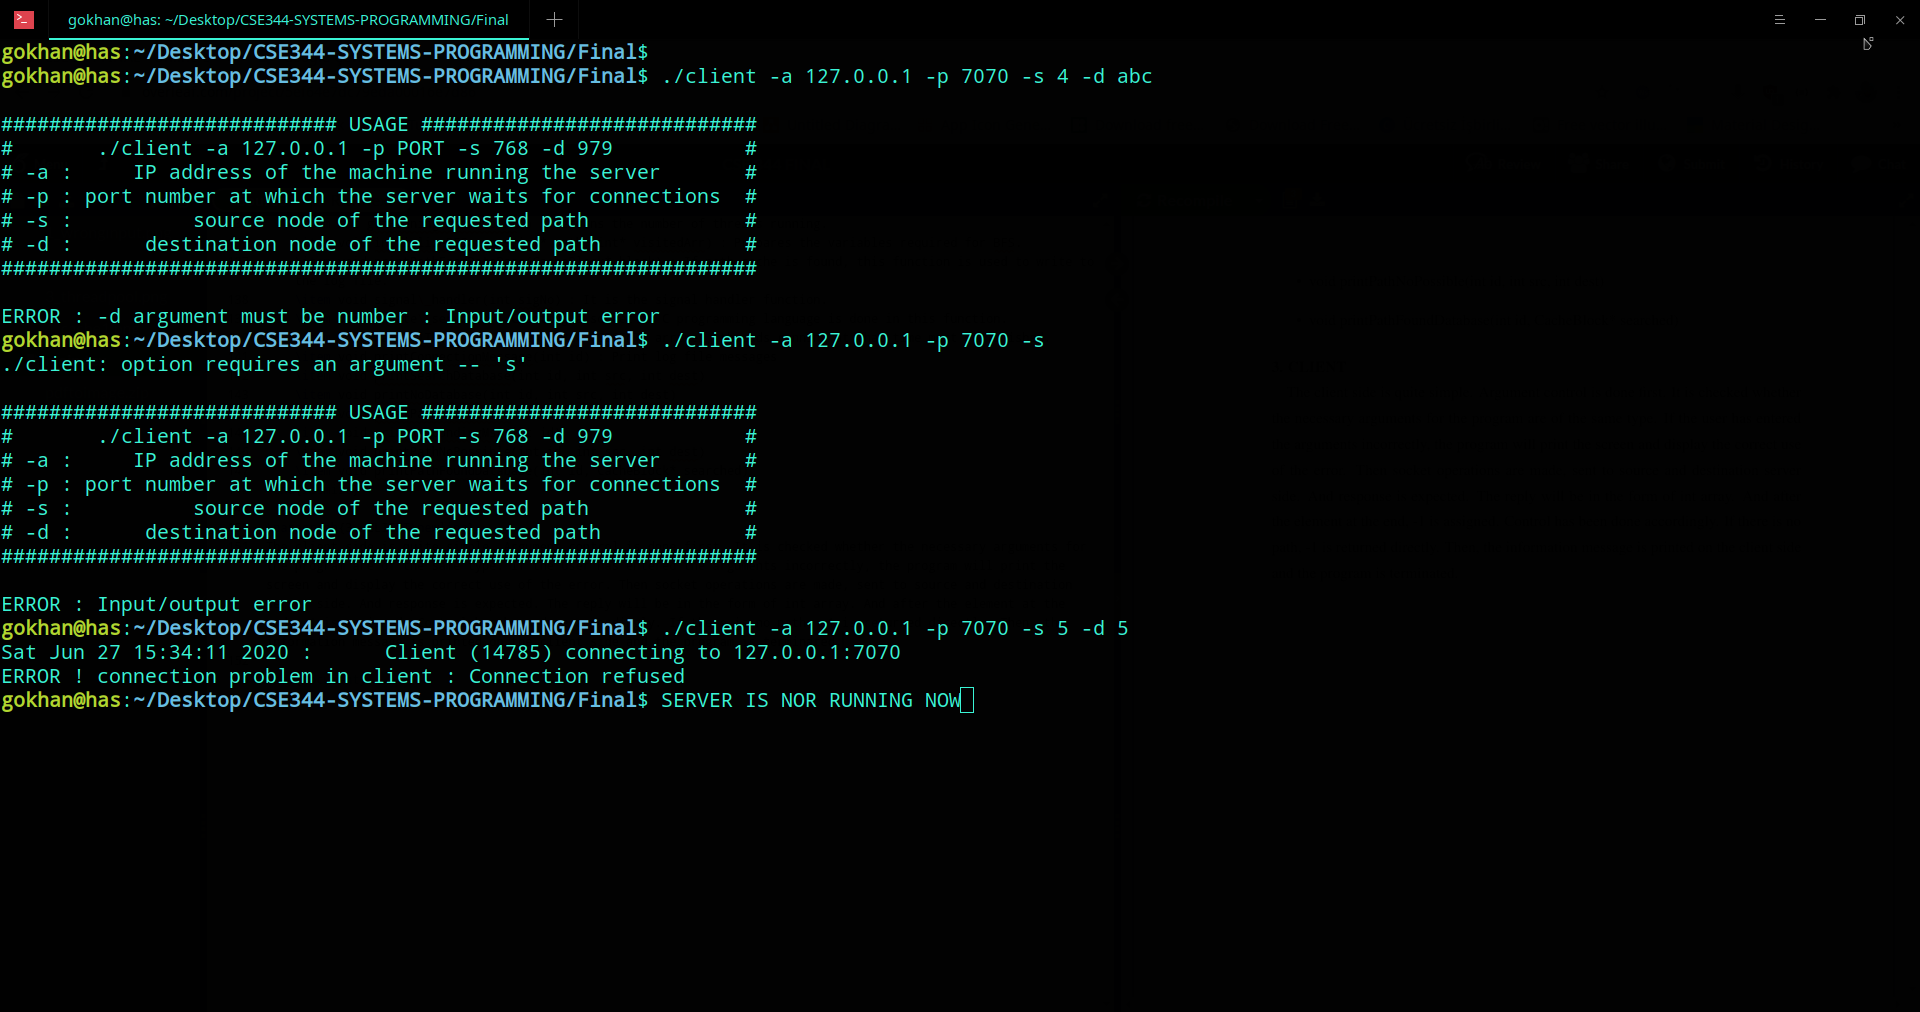
\includegraphics[scale=0.25]{5_client.png}
\caption{Wrong Input Test In Client}
\label{fig:compile}
\end{figure}

\paragraph{3.1 Used Functions In Client\newline}
\begin{itemize}
    \item int controlIfArgumentDigit(char* argumentValue) : Same arguments must be digit, fx portnumber, control these arguments.
    \item void errorExit(char* error) : Print error message and exit gracefully.
    \item void printUsage() : Print program usage if the user entered wrong input.
\end{itemize}

\newpage
\paragraph{4. OTHER USED FUNCTIONS IN HEADER FILES\newline}
\paragraph{4.1 graph.h\newline}
\begin{itemize}
    \item Graph* initializeGraph(int max) : Initializes graph by node number.
    \item void addEdge(Graph* graph, int source, int destination) : This function works when you want to add an edge to the graph.
    \item Graph* reinitializeGraph(Graph* oldGraph, int maxNumberNode) : It is written to re-initialize the graph when necessary.
    \item void freeGraph(Graph* \_graph) : The blocks separated by malloc for the graph structure are returned.
    \item void printGraph(Graph* graph) : It is written to understand whether the graph is properly read or not. It is not used in main.
\end{itemize}

\paragraph{4.2 queue.h\newline}
\begin{itemize}
    \item void initializeQueue(Queue* queue) : Queue is initialized according to the initial values.
    \item void push(Queue* queue, int element) : Adding an element to the end of the queue. Since the last node is held, it is added in O (1) time.
    \item int pop(Queue* queue) : Extracts an element from the queue. And it returns that element. Since the first node is held, the element is removed in O (1) time.
    \item void freeQueue(Queue* queue) : Resources used for the queue are free.
    \item void printPathQueue(Queue* queue, FILE* fileptr) : Queue elements are printed in sequence.
\end{itemize}

\newpage
\paragraph{4.3 cache.h\newline}
\begin{itemize}
    \item void initializeCache(CacheEntry* cacheEntryArr, int size) : Assigns initial values to all elements of the cache array.
    \item void addLast(CacheEntry* cacheEntryArr, Queue* pathx) : This function works when an element is added to the cache. Necessary information is taken from Queue * as a parameter.    
    \item void freeCache(CacheEntry* cacheEntryArr) : All resources used by cache are free.
    \item CacheBlock* searchCache(CacheEntry* cacheEntryArr, int source, int destination) : It is used in the case of searching for a path in cache. Returns the data structure of type CacheBlock *. Path is printed and send to from this structure.
    \item void printCacheBlock(CacheBlock* block) : In the cache, it is written for control purposes to understand whether the elements are added properly or not.
\end{itemize}

\paragraph{5. IMPORTANT NOTES\newline}
\begin{itemize}
    \item If you get a warning like the picture below while performing the valgrind test, the error will go away when you run the place I marked in the red box by adding it to the valgrind argument. Not all kinds of memory leak. Only errors are given.
    \begin{figure}[h!]
    \centering
    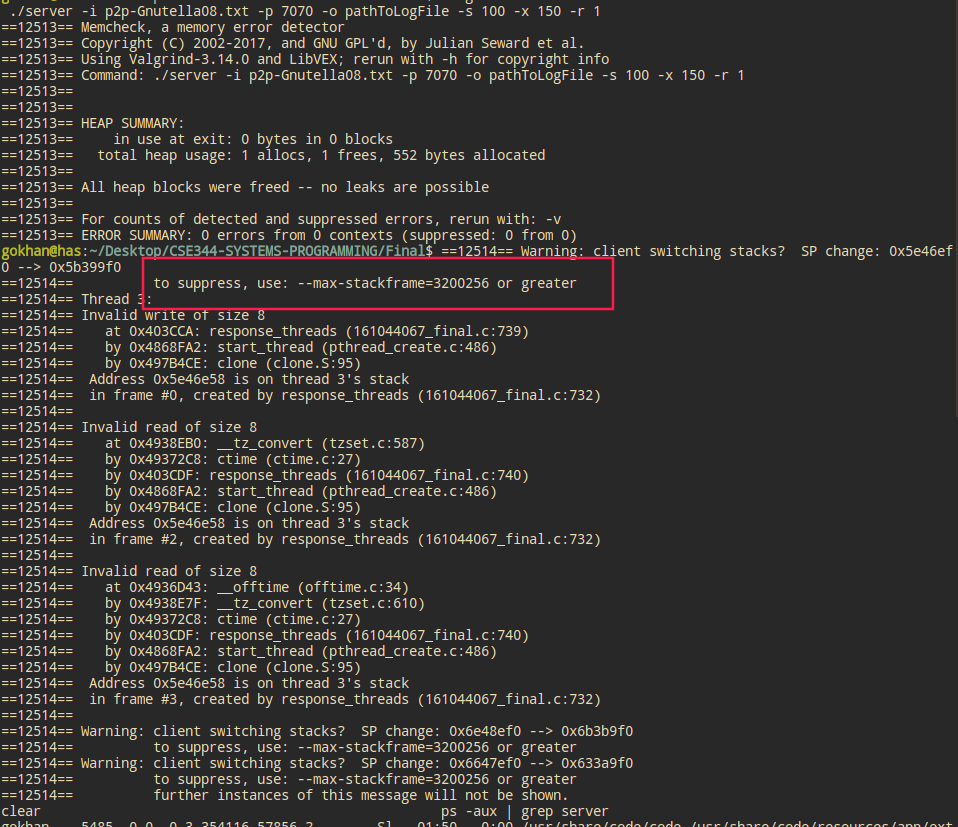
\includegraphics[scale=0.3]{6_walgrind_warnings.png}
    \caption{You can see screenshot in directory}
    \label{fig:compile}
    \end{figure}
\end{itemize}

\begin{figure}[h!]
\centering
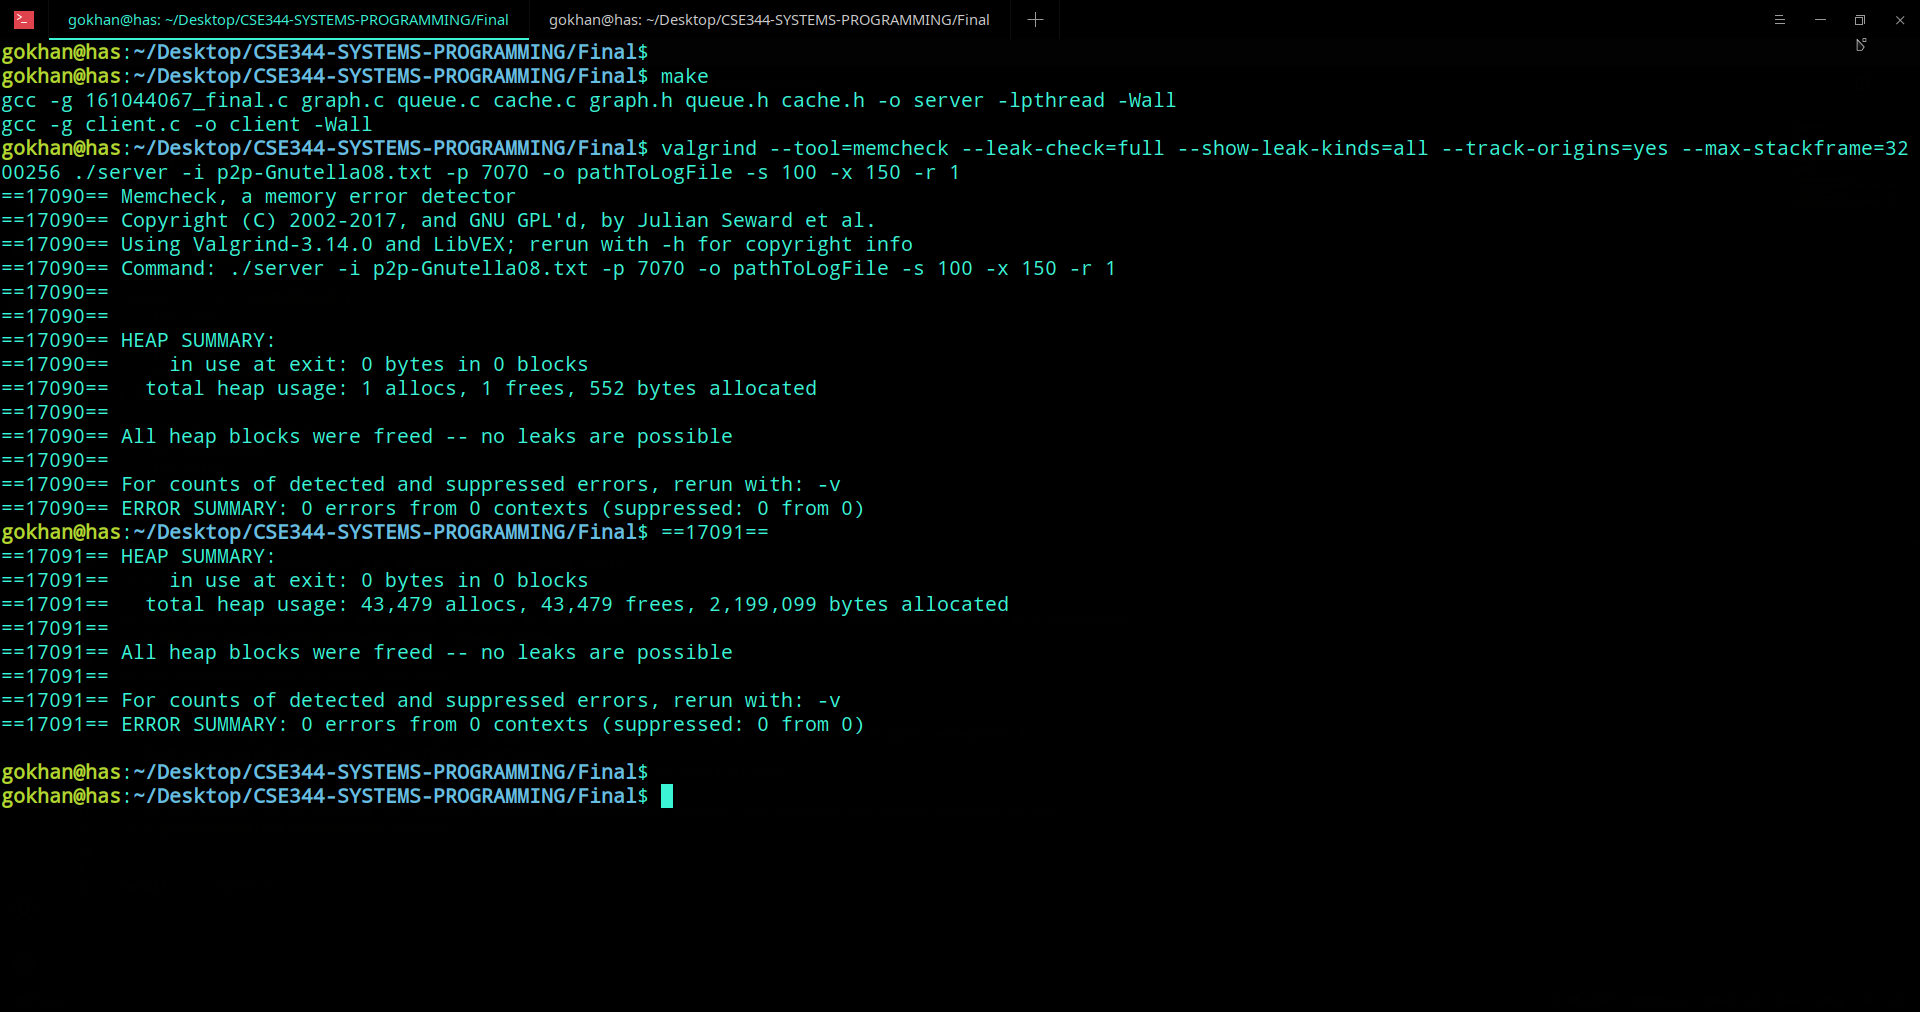
\includegraphics[scale=0.3]{7_memoryleak.png}
\caption{Memory Leak Test In Server}
\label{fig:compile}
\end{figure}

\begin{figure}[h!]
\centering
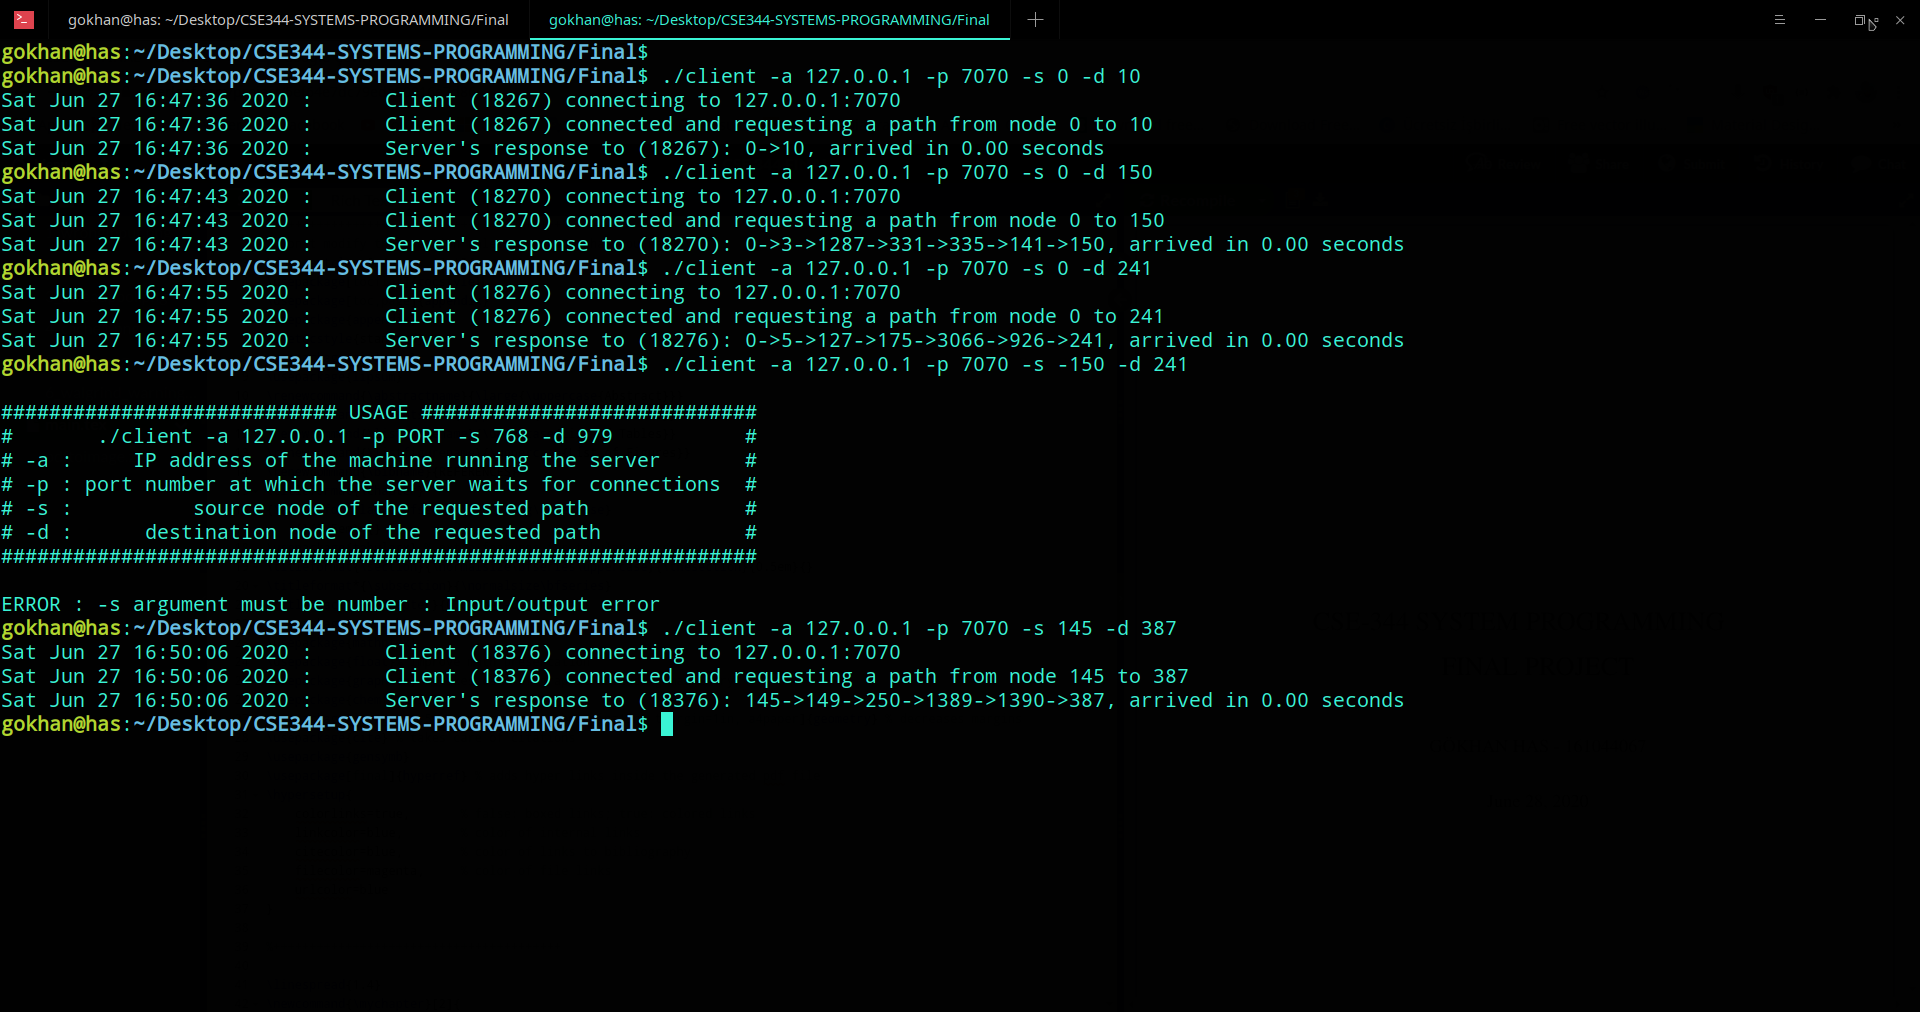
\includegraphics[scale=0.3]{8_clientside.png}
\caption{Sample Client Examples}
\label{fig:compile}
\end{figure}

\end{document}
